\documentclass[sigconf,edbt,table]{acmart-edbt2021}

\def\BibTeX{{\rm B\kern-.05em{\sc i\kern-.025em b}\kern-.08em
    T\kern-.1667em\lower.7ex\hbox{E}\kern-.125emX}}

\usepackage{booktabs} % For formal tables
\usepackage{tikz}
\usepackage[noend]{algpseudocode}
\usepackage{algorithm}
\usepackage{algorithmicx}
\usepackage{xcolor}
\usepackage{balance}

\usepackage{multirow}

%\usepackage{colortbl}
\usepackage{subcaption}
\usepackage{listings}
\usepackage{extarrows}
\usetikzlibrary{shapes,shapes.geometric,fit,automata,positioning}
\usetikzlibrary{decorations.pathmorphing}
\tikzset{snake it/.style={decorate, decoration=snake}}

%\definecolor{lightgray}{gray}{0.9}

\newcommand{\cho}[1]{{\color{red} #1}}

% Copyright
\setcopyright{rightsretained}

% DOI
\acmDOI{}

% ISBN
\acmISBN{978-3-89318-084-4}

%Conference
\acmConference[EDBT 2021]{24th International Conference on Extending Database Technology (EDBT)}{March 23-26, 2021}{Nicosia, Cyprus}
\acmYear{2021}

\settopmatter{printacmref=false, printccs=false, printfolios=false}

\pagestyle{empty} % removes running headers

% Math square brackets
\DeclareMathOperator{\rank}{rank}
\makeatletter
\newenvironment{sqcases}{%
  \matrix@check\sqcases\env@sqcases
}{%
  \endarray\right.%
}
\def\env@sqcases{%
  \let\@ifnextchar\new@ifnextchar
  \left\lbrack
  \def\arraystretch{1.2}%
  \array{@{}l@{\quad}l@{}}%
}
\makeatother

% Footnote reference
\makeatletter
\newcommand\footnoteref[1]{\protected@xdef\@thefnmark{\ref{#1}}\@footnotemark}
\makeatother

\newcommand\gsv[2]{{\color{red}{#1}( {#2} $^{\text{gsv}}$)}}
\newcommand\simpleton[1]{{\color{blue}{#1}}}

\tikzset{elliptic state/.style={draw,ellipse}}

\begin{document}
\title{Multiple-Source Context-Free Path Querying in Terms of Linear Algebra}
% \begin{document}
% \title{Implementing support for context-free path queering for the Cypher extension in RedisGraph}
% \titlenote{Produces the permission block, and copyright information}
% \subtitle{Extended Abstract}
% \subtitlenote{The full version of the author's guide is available as
%   \texttt{acmart.pdf} document}



\author{Arseniy Terekhov}
	\email{simpletondl@yandex.ru}
	\affiliation{
		\institution{Information Technologies, Mechanics and Optics University}
% 		\streetaddress{7/9 Universitetskaya nab.}
		% \city{St. Petersburg}
		% \country{Russia}
% 		\postcode{199034}
	}
	\affiliation{
		\institution{JetBrains Research}
		\streetaddress{Primorskiy prospekt 68-70, Building 1}
		\city{St. Petersburg}
		\country{Russia}
		\postcode{199034}
	}

\author{Vlada Pogozhelskaya}
	\email{pogozhelskaya@gmail.com}
	\affiliation{%
		\institution{Saint Petersburg State University}
		\streetaddress{7/9 Universitetskaya nab.}
		\city{St. Petersburg}
		\country{Russia}
		\postcode{199034}
	}

\author{Vadim Abzalov}
	\email{vadim.i.abzalov@gmail.com}
	\affiliation{%
		\institution{Saint Petersburg State University}
		\streetaddress{7/9 Universitetskaya nab.}
		\city{St. Petersburg}
		\country{Russia}
		\postcode{199034}
	}

\author{Timur Zinnatulin}
	\email{teemychteemych@gmail.com}
	\affiliation{%
		\institution{Saint Petersburg State University}
		\streetaddress{7/9 Universitetskaya nab.}
		\city{St. Petersburg}
		\country{Russia}
		\postcode{199034}
	}

\author{Semyon Grigorev}
	\email{s.v.grigoriev@spbu.ru}
	\email{semyon.grigorev@jetbrains.com}
	\orcid{0000-0002-7966-0698}
	\affiliation{
		\institution{Saint Petersburg State University}
		\streetaddress{7/9 Universitetskaya nab.}
		% \city{St. Petersburg}
		% \country{Russia}
		\postcode{199034}
	}
	\affiliation{
		\institution{JetBrains Research}
		\streetaddress{Primorskiy prospekt 68-70, Building 1}
		\city{St. Petersburg}
		\country{Russia}
		\postcode{199034}
	}

% The default list of authors is too long for headers}
% \renewcommand{\shortauthors}{B. Trovato et al.}
\renewcommand{\shortauthors}{Arseniy Terekhov et al.}


\begin{abstract}
	Context-Free Path Querying (CFPQ) allows one to express path constraints in navigational graph queries as context-free grammars.
	Although there are many algorithms for CFPQ developed, no graph database provides full-stack support of CFPQ.
	The Azimov's CFPQ algorithm is applicable for real-world graph analyses, as shown by Arseniy Terekhov.
	In this work we provide a modification to Azimov's algorithm for multiple-source CFPQ which makes the algorithm more practical and eases the integration into RedisGraph graph database.
	We also implement a Cypher graph query language extension for context-free constraints.
	Thus we provide the first full-stack support of CFPQ for graph databases.
	Our evaluation shows that the provided solution is suitable for real-world graph analyses.
\end{abstract}

%
% % The code below should be generated by the tool at
% % http://dl.acm.org/ccs.cfm
% % Please copy and paste the code instead of the example below.
% %
\begin{CCSXML}
		<ccs2012>
		<concept>
			<concept_id>10002951.10002952.10003197.10010825</concept_id>
			<concept_desc>Information systems~Query languages for non-relational engines</concept_desc>
			<concept_significance>500</concept_significance>
		</concept>
		<concept>
			<concept_id>10003752.10003766.10003771</concept_id>
			<concept_desc>Theory of computation~Grammars and context-free languages</concept_desc>
			<concept_significance>500</concept_significance>
		</concept>
		<concept>
			<concept_id>10002950.10003624.10003633.10003640</concept_id>
			<concept_desc>Mathematics of computing~Paths and connectivity problems</concept_desc>
			<concept_significance>300</concept_significance>
		</concept>
		<concept>
			<concept_id>10002951.10002952.10002953.10010146</concept_id>
			<concept_desc>Information systems~Graph-based database models</concept_desc>
			<concept_significance>500</concept_significance>
		</concept>
		</ccs2012>
\end{CCSXML}

    \ccsdesc[500]{Information systems~Graph-based database models}
	\ccsdesc[500]{Information systems~Query languages for non-relational engines}
	\ccsdesc[500]{Theory of computation~Grammars and context-free languages}
    \ccsdesc[300]{Mathematics of computing~Paths and connectivity problems}


% \keywords{ACM proceedings, \LaTeX, text tagging}

%% A "teaser" image appears between the author and affiliation
%% information and the body of the document, and typically spans the
%% page.
%\begin{teaserfigure}
%  \includegraphics[width=\textwidth]{new_hope.png}
%  \caption{Episode IV: A New Hope}
%  \label{fig:teaser}
%\end{teaserfigure}

\maketitle

\section{Introduction}

Scalable high-performance graph analysis is an actual challenge.
There is a big number of ways to attack this challenge~\cite{Coimbra2021} and the first promising idea is to utilize general-purpose graphic processing units (GPGPU-s).
Such existing solutions, as CuSha~\cite{10.1145/2600212.2600227} and Gunrock~\cite{7967137} show that utilization of GPUs can improve the performance of graph analysis, moreover it is shown that solutions may be scaled to multi-GPU systems.
But low flexibility and high complexity of API are problems of these solutions.

The second promising thing which provides a user-friendly API for high-performance graph analysis algorithms creation is a GraphBLAS API~\cite{7761646} which provides linear algebra based building blocks to create graph analysis algorithms.
The idea of GraphBLAS is based on is a well-known fact that linear algebra operations can be efficiently implemented on parallel hardware.
Along with this, a graph can be natively represented using matrices: adjacency matrix, incidence matrix, etc.
While reference CPU-based implementation of GraphBLAS, SuiteSparse:GraphBLAS~\cite{10.1145/3322125}, demonstrates good performance in real-world tasks, GPU-based implementation is challenging.

One of the challenges in this way is that real data are often sparse, thus underlying matrices and vectors are also sparse, and, as a result, classical dense data structures and respective algorithms are inefficient. 
So, it is necessary to use advanced data structures and procedures to implement sparse linear algebra, but the efficient implementation of them on GPU is hard due to the irregularity of workload and data access patterns.
Though such well-known libraries as cuSparse show that sparse linear algebra operations can be efficiently implemented for GPGPU-s, it is not so trivial to implement GraphBLAS on GPGPU. 
First of all, it requires \textit{generic} sparse linear algebra, thus it is impossible just to reuse existing libraries which are almost all specified for operations over floats.
The second problem is specific optimizations, such as maskings fusion, which can not be natively implemented on top of existing kernels.
Nevertheless, there is a number of implementations of GraphBLAS on GPGPU, such as GraphBLAST:~\cite{yang2019graphblast}, GBTL~\cite{7529957}, which show that GPGPUs utilization can improve the performance of GraphBLAS-based graph analysis solutions.
But these solutions are not portable because they are based on Nvidia Cuda stack.
Moreover, the scalability problem is not solved: all these solutions support only single-GPU, not multi-GPU computations.

To provide portable GPU implementation of GraphBLAS API we developed a \textit{SPLA} library (sources are published on GitHub: \url{https://github.com/JetBrains-Research/spla}).
This library utilizes OpenCL for GPGPU computing to be portable across devices of different vendors.
Moreover, it is initially designed to utilize multiple GPGPUs to be scalable.
To sum up, the contribution of this work is the following.
\begin{itemize}
    \item Design of portable GPU GraphBLAS implementation proposed. The design involves the utilization of multipole GPUS. Additionally, the proposed design is aimed to simplify library tuning and wrappers for different high-level platforms and languages creation. 
    \item Subset of GraphBLAS API, including such operations as masking, matrix-matrix multiplication, matrix-matrix e-wise addition, is implemented. The current implementation is limited by COO and CSR matrix representation format and uses basic algorithms for some operations, but work in progress and more data formats will be supported and advanced algorithms will be implemented in the future.
    \item Preliminary evaluation on such algorithms as breadth-first search (BFS) and triangles counting (TC), and real-world graphs shows portability across different vendors and promising performance: for some problems Spla is comparable with GraphBLAST. Surprisingly, for some problems, the proposed solution on embedded Intel graphic card shows better performance than SuiteSparse:GraphBLAS on the same CPU. At the same time, the evaluation shows that further optimization is required.
\end{itemize} 
\section{Preliminaries}

We introduce !!!!

\subsection{Context-Free Path Querying}

Graph, grammar, etc.

Let $i\pi j$ denote a unique path between nodes $i$ and $j$ of the graph and $l(\pi)$ denotes a unique string which is obtained from the concatenation of edge labels along the path $\pi$.
For a context-free grammar $G = (\Sigma, N, P, S)$ and directed labelled graph $D = (Q, \Sigma, \delta)$, a triple $(A, i, j)$ is \textit{realizable} iff there is a path $i\pi j$ such that nonterminal $A \in N$ derives $l(\pi)$.

\subsection{Tensor-Based algorithm for CFPQ}

\begin{algorithm}[H]
\begin{algorithmic}[1]
\caption{Kronecker product context-free recognizer for graphs}
\label{alg:Kronecker}
\Function{contextFreePathQuerying}{D, G}
\EndFunction
\end{algorithmic}
\end{algorithm}

\subsection{Planar Graphs}

A planar graph $G = (V, E)$ is a graph that can be embedded in the plane.

Outer face - unbounded face in specific embedding.

Directed graph (\textit{digraph})

...

\subsection{Dynamic reachability algorithms}

We consider algorithms that solve the problem of reachability in planar directed graphs. In the \textit{dynamic reachability problem} we are given a graph $G$ subject to edge updates (insertions or deletions) and the goal is to design a data structure that would allow answering queries about the existence of a path.

We need to answer the queries of type: "Is there a directed path from $u$ to $v$ in $G$?". If vertex $u$ in all the queries is fixed we say that algorithm is \textit{single-source}. It is said to be \textit{all-pairs} if vertices $u, v$ can be any vertices of planar digraph $G$, in this case it can be also called \textit{dynamic transitive closure}.

We say that the algorithm is \textit{fully dynamic} if it supports both additions and deletions of edges. It is said to be \textit{semi dynamic} if it supports only one of these updates. If semi dynamic algorithm supports additions only it is called \textit{incremental}, if deletions only - \textit{decremental}.






\section{Matrix-based multiple-source CFPQ algorithm}
\label{sec:multiple-source-algo}

 In this section we introduce two versions of the multiple-source matrix-based CFPQ algorithm.
 This algorithm is a modification of Azimov's matrix-based algorithm for CFPQ and its core idea is to cut off those vertices which are not in the selected set of start vertices.


In order to simplify Azimov's algorithm modification and the final algorithm description, we assume the input graph to have only edge labels.
Note, that we always can convert the original graph into such form.
To do it, we should add loops into vertices in the following way: for the vertex $i$ we add an edge $i \xrightarrow{x} i$ iff $\lambda_V(i) = x$ and $x\neq \varnothing$.
This way we can switch to an edge-labeled graph with the same number of vertices while preserving the defined semantics of CFPQ.

\begin{figure}[h]
    \centering
    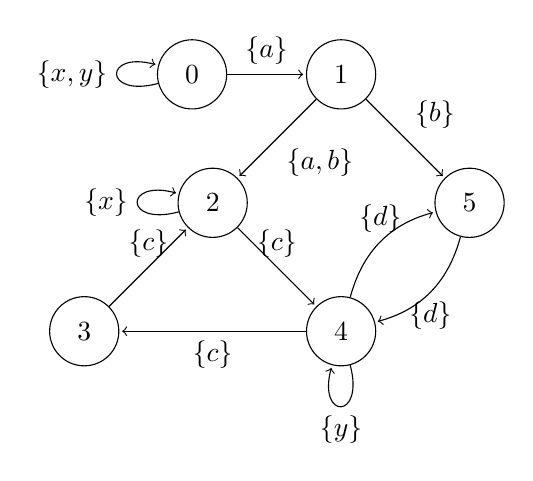
\begin{tikzpicture}[shorten >=1pt,auto]
       \node[state] (q_0)                        {$0$};
       \node[state] (q_1) [right=of q_0]         {$1$};
       \node[state] (q_2) [below left=of q_1]    {$2$};
       \node[state] (q_3) [below left=of q_2]    {$3$};
       \node[state] (q_4) [below right=of q_2]   {$4$};
       \node[state] (q_5) [below right=of q_1]   {$5$};
       \path[->]
        (q_0) edge[loop left]  node {$\{x, y\}$} (q_0)
        (q_0) edge  node {$\{a\}$} (q_1)
        (q_2) edge[loop left]  node {$\{x\}$} (q_2)
        (q_1) edge  node {$\{b\}$} (q_5)
        (q_1) edge  node {$\{a, b\}$} (q_2)
        (q_3) edge[above]  node {$\{c\}$} (q_2)
        (q_4) edge  node {$\{c\}$} (q_3)
        (q_2) edge[above]  node {$\{c\}$} (q_4)
        (q_4) edge[loop below]  node {$\{y\}$} (q_4)
        (q_5) edge[bend left, below]  node {$\{d\}$} (q_4)
        (q_4) edge[bend left, above]  node {$\{d\}$} (q_5);
    \end{tikzpicture}
    \caption{The example of $D_1'$: the modified input graph $D_1$}
    \label{fig:example_modified_input_graph}
\end{figure}

The adjacency matrix $M$ of the graph $D_1'$ is
{
    \renewcommand{\arraystretch}{0.7}
    \setlength\arraycolsep{2pt}
$$
    M =
    \begin{pmatrix}
    \{x, y\}     & \{a\}       & \varnothing & \varnothing & \varnothing & \varnothing \\
    \varnothing  & \varnothing & \{a, b\}    & \varnothing & \varnothing & \{b\}       \\
    \varnothing  & \varnothing & \{x\}       & \varnothing & \{c\}       & \varnothing \\
    \varnothing  & \varnothing & \{c\}       & \varnothing & \varnothing & \varnothing \\
    \varnothing  & \varnothing & \varnothing & \{c\}       & \{y\}       & \{d\}       \\
    \varnothing  & \varnothing & \varnothing & \varnothing & \{d\}       & \varnothing
    \end{pmatrix}.
$$
}
Note that this transformation is impractical for real-world graphs, thus we use it only for algorithm description.

The first version of multiple-source algorithm is the Azimov's algorithm equipped with vertices filtering.
Let $G = (N, \Sigma, P, S)$ be the input context-free grammar, $D = (V, E, \Sigma_V, \Sigma_E, \lambda_V, \lambda_E)$ be the input graph and $Src$ be the input set of start vertices.
The result of the algorithm is a Boolean matrix which represents relation $R_{S,D}^{Src}$.

\begin{algorithm}
\small
\begin{algorithmic}[1]
\caption{Multiple-source context-free path querying algorithm}
\label{alg:algo1}
\Function{MultiSrcCFPQNaive}{\par
\hskip\algorithmicindent $D = (V, E, \Sigma_V, \Sigma_E, \lambda_V, \lambda_E)$, \par
\hskip\algorithmicindent $G=(N,\Sigma,P,S)$, \par
\hskip\algorithmicindent
$Src$}
    \State{$T \gets \{T^A \mid  A \in N, T^A[i,j] \gets \textit{false} \text{, for all $i,j$}\} $}

    \State{$TSrc \gets \{TSrc^A \mid  A \in N, TSrc^A[i,j] \gets \textit{false} \text{, for all $i,j$}\}$}

    \ForAll{$ v \in Src$} \Comment{Input matrix initialization}
        \State{$TSrc^S[v,v] \gets true$}
    \EndFor
    
    \State $MSrc \gets TSrc^S$

    \ForAll{$A \to x \in P$} \Comment{Simple rules initialization}
        \ForAll{$(v, to) \in E, \lambda_E(v,to) = x$}
            \State{$T^A[v,to] \gets true$}
        \EndFor
    \EndFor

    \While{$T\ or\ TSrc\ is\ changing$} \Comment{Algorithm's body}
        \ForAll{$A \to B C \in P$}
            \State{$M \gets TSrc^A*T^B$}
            \State{$T^A \gets T^A + M*T^C$}
            \State{$TSrc^B \gets TSrc^B + TSrc^A$}
            \State{$TSrc^C \gets TSrc^C + $ \Call{getDst}{$M$}}
        \EndFor
    \EndWhile
    \State \Return $MSrc * T^S$
\EndFunction



\Function{getDst}{$M$}
    \State{$A[i,j] \gets \textit{false}$}
    \ForAll{$(v,to) \in V^2 \mid M[v,to] = true$}
        \State{$A[to,to] \gets true$}
    \EndFor
    \State \Return A
\EndFunction
\end{algorithmic}
\end{algorithm}

In order to solve the single-source and multiple-source CFPQ problem, we modified the Azimov's algorithm.
Each time, when a grammar rule is applied (see line \textbf{8} of Algorithm~\ref{alg:algo0}: Boolean matrix multiplication $T^A = T^A + T^B \cdot T^C$ for each $A \rightarrow BC \in P$), only vertices of interest should be stored.
To do it, we added one more matrix multiplication: $T^A = T^A + (TSrc^A \cdot T^B) \cdot T^ C$, where $TSrc^A$---matrix of start vertices for the current iteration (lines \textbf{11-13} of the Algorithm~\ref{alg:algo1}).
In the end of every iteration of for loop, it is necessary to update the set of source vertices paths from which we need to calculate.
To do it, the we call the function \textsc{getDst} (see lines \textbf{17-21}), in line \textbf{15}.
Thus, the modified algorithm supports the frontier of the vertices of interest and updates it on each iteration.
As a result, it only computes the paths which starts from the small set of selected vertices.

In case when one has a sequence of similar queries to the single graph, it may be useful to cache results of the query evaluation and share them between queries.
This may help to avoid recalculation of the already computed results.
To introduce sharing of results between queries, we modify the previous version of the algorithm.
The modified version stores all the vertices the paths from which have already been calculated in cache \textit{index}, which is used to filter such vertices in line \textbf{11} of Algorithm~\ref{alg:algo2}.
Thus, the modified algorithm calculates paths from the particular vertex only once.
Note, that \textsc{CreateIndex} function should be called first, and the created index can be shared between multiple calls of \textsc{MultiSrcCFPQCache} after that.

\begin{algorithm}
\small
\begin{algorithmic}[1]
\caption{Multiple-source context-free path querying algorithm with caching}
\label{alg:algo2}
\Function{CreateIndex}{ \par
\hskip\algorithmicindent $D = (V, E, \Sigma_V, \Sigma_E, \lambda_V, \lambda_E)$, \par
\hskip\algorithmicindent $G=(N,\Sigma,P,S)$}
    \State{$T \gets \{T^A \mid  A \in N, T^A[i,j] \gets \textit{false} \text{, for all $i,j$}\}$}

    \State{$TSrc \gets \{TSrc^A \mid  A \in N, TSrc^A[i,j] \gets \textit{false} \text{, for all $i,j$}\}$}

    \ForAll{$A \to x \in P$} \Comment{Simple rules initialization}
        \ForAll{$(v, to) \in E, \lambda_E(v,to) = x$}
            \State{$T^A[v,to] \gets \textit{true}$}
        \EndFor
    \EndFor

    \State \Return $(T, TSrc)$
\EndFunction
\State
\Function{MultiSrcCFPQCache}{ \par
\hskip\algorithmicindent $D = (V, E, \Sigma_V, \Sigma_E, \lambda_V, \lambda_E)$, \par
\hskip\algorithmicindent $G=(N,\Sigma,P,S)$, \par
\hskip\algorithmicindent $Src$, \par
\hskip\algorithmicindent $Index = (T, TSrc)$}

    \State{$TNewSrc \gets \{TNewSrc^A \mid  A \in N, TNewSrc^A \gets \textit{false} \text{, for all $i,j$}\}\}$}

    \ForAll{$v \in Src \mid TSrc[v,v] = false$}
        \State{$TNewSrc^S[v,v] \gets true$}
    \EndFor
    
    \State $MSrc \gets TNewSrc^S$

    \While{\textit{T or TNewSrc is changing}}
        \ForAll{$A \to B C \in P$}
            \State{$M \gets TNewSrc^A*T^B$}
            \State{$T^A \gets T^A + M*T^C$}

            \State{$TNewSrc^B \gets TNewSrc^B + TNewSrc^A \setminus TSrc^B$}
            \State{$TNewSrc^C \gets TNewSrc^C + $ \Call{getDst}{M}} $\setminus$ $TSrc^C$
        \EndFor
    \EndWhile
    \State \Return $MSrc*T^S$
    \Comment{We want to return only relevant data, not all cached results}
\EndFunction


\end{algorithmic}
\end{algorithm}


\subsection{Example}

Consider the first few steps of the proposed algorithm (without caching) on the graph $D_1'$, grammar $G_1^{\text{wcnf}}$, and the set of start vertices $Src = \{2\}$.
At the first step (lines \textbf{4}--\textbf{5}) $TSrc^S[2,2]$ sets to \textit{true}, all other cells have value \textit{false}.
Then the set of matrices $T$ is initialized using rules $C \to c, D \to d, Y \to y$ as follows:
{
    \renewcommand{\arraystretch}{0.7}
    \setlength\arraycolsep{2pt}
\begin{align*}
    T^C& = \mathcal{E}^c =
    \begin{pmatrix}
    . & . & . & . & . & . \\
    . & . & . & . & . & . \\
    . & . & . & . & 1 & . \\
    . & . & 1 & . & . & . \\
    . & . & . & 1 & . & . \\
    . & . & . & . & . & .
\end{pmatrix},
    T^D = \mathcal{E}^d =
    \begin{pmatrix}
    . & . & . & . & . & . \\
    . & . & . & . & . & . \\
    . & . & . & . & . & . \\
    . & . & . & . & . & . \\
    . & . & . & . & . & 1 \\
    . & . & . & . & 1 & .
\end{pmatrix},\\
    T^Y& = \mathcal{V}^y =
    \begin{pmatrix}
    1 & . & . & . & . & . \\
    . & . & . & . & . & . \\
    . & . & . & . & . & . \\
    . & . & . & . & . & . \\
    . & . & . & . & 1 & . \\
    . & . & . & . & . & .
\end{pmatrix}
\end{align*}
}

The following computations take place at the first iteration of the while loop in line~\textbf{9} for the grammar rule $S \to C E$.
First, the matrix $M$ is computed as follows
{
    \renewcommand{\arraystretch}{0.7}
    \setlength\arraycolsep{2pt}
\begin{align*}
M=TSrc^S*T^C =
\begin{pmatrix}
    . & . & . & . & . & . \\
    . & . & . & . & . & . \\
    . & . & 1 & . & . & . \\
    . & . & . & . & . & . \\
    . & . & . & . & . & . \\
    . & . & . & . & . & .
\end{pmatrix}*
\begin{pmatrix}
    . & . & . & . & . & . \\
    . & . & . & . & . & . \\
    . & . & . & . & 1 & . \\
    . & . & 1 & . & . & . \\
    . & . & . & 1 & . & . \\
    . & . & . & . & . & .
\end{pmatrix}=
\begin{pmatrix}
    . & . & . & . & . & . \\
    . & . & . & . & . & . \\
    . & . & . & . & 1 & . \\
    . & . & . & . & . & . \\
    . & . & . & . & . & . \\
    . & . & . & . & . & .
\end{pmatrix}
\end{align*}
}

Since matrix $T^E$ is empty, $T^S$ stays the same in line~\textbf{12}, as well as $TSrc^C$ in line~\textbf{13}.
But the matrix $TSrc^E$ is updated (line~\textbf{14}):
{
    \renewcommand{\arraystretch}{0.7}
    \setlength\arraycolsep{2pt}
\begin{align*}
&TSrc^E = TSrc^E + \textsc{getDist}(M) = \\ &=
\begin{pmatrix}
    . & . & . & . & . & . \\
    . & . & . & . & . & . \\
    . & . & . & . & . & . \\
    . & . & . & . & . & . \\
    . & . & . & . & . & . \\
    . & . & . & . & . & .
\end{pmatrix} +
\begin{pmatrix}
    . & . & . & . & . & . \\
    . & . & . & . & . & . \\
    . & . & . & . & . & . \\
    . & . & . & . & . & . \\
    . & . & . & . & 1 & . \\
    . & . & . & . & . & .
\end{pmatrix}=
\begin{pmatrix}
    . & . & . & . & . & . \\
    . & . & . & . & . & . \\
    . & . & . & . & . & . \\
    . & . & . & . & . & . \\
    . & . & . & . & 1 & . \\
    . & . & . & . & . & .
\end{pmatrix}
\end{align*}
}

This means that we are interested in paths that start from the vertex 4 and satisfy the constraints specified by nonterminal $E$.

The second rule is $S \to C S_1$ and its processing is similar to previous one.
After processing,
{
    \renewcommand{\arraystretch}{0.7}
    \setlength\arraycolsep{2pt}
\begin{align*}
TSrc^{S_1} =
\begin{pmatrix}
    . & . & . & . & . & . \\
    . & . & . & . & . & . \\
    . & . & . & . & . & . \\
    . & . & . & . & . & . \\
    . & . & . & . & 1 & . \\
    . & . & . & . & . & .
\end{pmatrix},
\end{align*}
}

The third rule is $E \to Y D$.
Here $M$ is computed as follows:
{
    \renewcommand{\arraystretch}{0.7}
    \setlength\arraycolsep{2pt}
\begin{align*}
M = TSrc^E * T^Y =
\begin{pmatrix}
    . & . & . & . & . & . \\
    . & . & . & . & . & . \\
    . & . & . & . & . & . \\
    . & . & . & . & . & . \\
    . & . & . & . & 1 & . \\
    . & . & . & . & . & .
\end{pmatrix}*
\begin{pmatrix}
    1 & . & . & . & . & . \\
    . & . & . & . & . & . \\
    . & . & . & . & . & . \\
    . & . & . & . & . & . \\
    . & . & . & . & 1 & . \\
    . & . & . & . & . & .
\end{pmatrix}=
\begin{pmatrix}
    . & . & . & . & . & . \\
    . & . & . & . & . & . \\
    . & . & . & . & . & . \\
    . & . & . & . & . & . \\
    . & . & . & . & 1 & . \\
    . & . & . & . & . & .
\end{pmatrix}
\end{align*}
}

Then the algorithm updates $T^E$ as follows:

{
    \renewcommand{\arraystretch}{0.7}
    \setlength\arraycolsep{2pt}
\begin{align*}
&T^E = T^E + M * T^D = \\ &=
\begin{pmatrix}
    . & . & . & . & . & . \\
    . & . & . & . & . & . \\
    . & . & . & . & . & . \\
    . & . & . & . & . & . \\
    . & . & . & . & . & . \\
    . & . & . & . & . & .
\end{pmatrix}+
\begin{pmatrix}
    . & . & . & . & . & . \\
    . & . & . & . & . & . \\
    . & . & . & . & . & . \\
    . & . & . & . & . & . \\
    . & . & . & . & 1 & . \\
    . & . & . & . & . & .
\end{pmatrix}*
\begin{pmatrix}
    . & . & . & . & . & . \\
    . & . & . & . & . & . \\
    . & . & . & . & . & . \\
    . & . & . & . & . & . \\
    . & . & . & . & . & 1 \\
    . & . & . & . & 1 & .
\end{pmatrix}=
\begin{pmatrix}
    . & . & . & . & . & . \\
    . & . & . & . & . & . \\
    . & . & . & . & . & . \\
    . & . & . & . & . & . \\
    . & . & . & . & . & 1 \\
    . & . & . & . & . & .
\end{pmatrix}
\end{align*}
}

Thus we know that there exists a path from vertex 4 to vertex 5 such that it forms a word derivable from $E$.

The last rule is $S_1 \to S D$.
During processing this rule only $TSrc^S$ is updated, since $T^S$ is empty:
{
    \renewcommand{\arraystretch}{0.7}
    \setlength\arraycolsep{2pt}
\begin{align*}
&TSrc^S = TSrc^S + TSrc^{S_1} = \\ &=
\begin{pmatrix}
    . & . & . & . & . & . \\
    . & . & . & . & . & . \\
    . & . & 1 & . & . & . \\
    . & . & . & . & . & . \\
    . & . & . & . & . & . \\
    . & . & . & . & . & .
\end{pmatrix}*
\begin{pmatrix}
    . & . & . & . & . & . \\
    . & . & . & . & . & . \\
    . & . & . & . & . & . \\
    . & . & . & . & . & . \\
    . & . & . & . & 1 & . \\
    . & . & . & . & . & .
\end{pmatrix}=
\begin{pmatrix}
    . & . & . & . & . & . \\
    . & . & . & . & . & . \\
    . & . & 1 & . & . & . \\
    . & . & . & . & . & . \\
    . & . & . & . & 1 & . \\
    . & . & . & . & . & .
\end{pmatrix}
\end{align*}
}

This is the end of the first iteration.

At the second iteration, matrices $M$ and then $T^S$ are computed for rule $S \to C E$ as follows:
{
    \renewcommand{\arraystretch}{0.7}
    \setlength\arraycolsep{2pt}
\begin{align*}
&M = TSrc^S * T^C =
\begin{pmatrix}
    . & . & . & . & . & . \\
    . & . & . & . & . & . \\
    . & . & 1 & . & . & . \\
    . & . & . & . & . & . \\
    . & . & . & . & 1 & . \\
    . & . & . & . & . & .
\end{pmatrix} *
\begin{pmatrix}
    . & . & . & . & . & . \\
    . & . & . & . & . & . \\
    . & . & . & . & 1 & . \\
    . & . & 1 & . & . & . \\
    . & . & . & 1 & . & . \\
    . & . & . & . & . & .
\end{pmatrix}=
\begin{pmatrix}
    . & . & . & . & . & . \\
    . & . & . & . & . & . \\
    . & . & . & . & 1 & . \\
    . & . & . & . & . & . \\
    . & . & . & 1 & . & . \\
    . & . & . & . & . & .
\end{pmatrix}
\\
&T^S = M * T^E =
\begin{pmatrix}
    . & . & . & . & . & . \\
    . & . & . & . & . & . \\
    . & . & . & . & 1 & . \\
    . & . & . & . & . & . \\
    . & . & . & 1 & . & . \\
    . & . & . & . & . & .
\end{pmatrix} *
\begin{pmatrix}
    . & . & . & . & . & . \\
    . & . & . & . & . & . \\
    . & . & . & . & . & . \\
    . & . & . & . & . & . \\
    . & . & . & . & . & 1 \\
    . & . & . & . & . & .
\end{pmatrix} =
\begin{pmatrix}
    . & . & . & . & . & . \\
    . & . & . & . & . & 1 \\
    . & . & . & . & . & . \\
    . & . & . & . & . & . \\
    . & . & . & . & . & . \\
    . & . & . & . & . & .
\end{pmatrix}
\end{align*}
}

Thus, we found the first path that satisfies our query.
After all iterations finished, we get the final result:
{
    \renewcommand{\arraystretch}{0.7}
    \setlength\arraycolsep{2pt}
\begin{align*}
T^S =
\begin{pmatrix}
    . & . & . & . & . & . \\
    . & . & . & . & 1 & 1 \\
    . & . & . & . & . & . \\
    . & . & . & . & . & . \\
    . & . & . & . & . & . \\
    . & . & . & . & . & .
\end{pmatrix}
\end{align*}
}
Thus only vertices 4 and 5 are reachable from the vertex 2 by a path which forms a word derivable from the start nonterminal $S$.

\subsection{Implementation Notes}

All of the versions presented have been implemented$\footnote{GitHub repository with implemented algorithms: \url{https://github.com/JetBrains-Research/CFPQ_PyAlgo}, last accessed 28.08.2020}$ using GraphBLAS framework that allows one to represent graphs as matrices and to work with them in terms of linear algebra.
For~convenience, the code is written in Python using pygraphblas\footnote{GitHub repository of PyGraphBLAS library: \url{https://github.com/michelp/pygraphblas}}, which is a Python wrapper for GraphBLAS API and is based on SuiteSparse:GraphBLAS\footnote{GitHub repository of SuiteSparse:GraphBLAS library: \url{https://github.com/DrTimothyAldenDavis/SuiteSparse}}~\cite{10.1145/3322125} --- the complete implementation of the GraphBLAS standard.
This library is specialized to work with sparse matrices which appear in real graphs most often.

\subsection{Algorithm Evaluation}\label{sect:py_algo_evaluation}

We evaluate both described versions of the multiple-source algorithm on real-world graphs.
For evaluation, we use a PC with Ubuntu 20.04 installed.
It has Intel core i7-4790 CPU, 3.60GHz, and DDR3 32Gb RAM.
As far as we evaluate only the execution time of the algorithm, we store each graph fully in RAM as its adjacency matrix in sparse format.
Note, that graph loading time is not included in the result time of evaluation.

For evaluation we use graphs and queries from CFPQ\_Data dataset\footnote{CFPQ\_Data is a dataset for CFPQ evaluation which contains both synthetic and real-world data and queries \url{https://github.com/JetBrains-Research/CFPQ\_Data}, last accessed 28.08.2020.}.
Detailed information, such as the number of vertices and edges, and the number of edges with the specific label, on graphs used in evaluation is provided in table~\ref{tbl:graphs_for_cfpq}.
We use classical same-generation queries $g_1$~(eq.~\ref{eqn:g_1}) and $g_2$~(eq.~\ref{eqn:g_2}) which are used in other works for CFPQ evaluation.
We also use $geo$~(eq.~\ref{eqn:geo}) query provided by Jochem Kuijpers et. al~\cite{Kuijpers:2019:ESC:3335783.3335791} for \textit{geospecies} RDF.
Note that in queries we use $\overline{x}$ notation to denote the inverse of the $x$ relation and the respective edge.

\begin{align}
\begin{split}
\label{eqn:g_1}
S \to & \overline{\textit{subClassOf}} \ \ S \ \textit{subClasOf} \mid \overline{\textit{type}} \ \ S \ \textit{type}\\   & \mid \overline{\textit{subClassOf}} \ \ \textit{subClassOf} \mid \overline{\textit{type}} \ \textit{type}
\end{split}
\end{align}
\begin{align}
\label{eqn:g_2}
S \to \overline{\textit{subClassOf}} \ \ S \ \textit{subClasOf} \mid \textit{subClassOf}
\end{align}
\begin{align}
\begin{split}
\label{eqn:geo}
S \to & \textit{broaderTransitive} \ \  S \ \overline{\textit{broaderTransitive}} \\
      & \mid \textit{broaderTransitive} \ \  \overline{\textit{broaderTransitive}}
\end{split}
\end{align}

{\setlength{\tabcolsep}{0.1em}
\begin{table}
{
\caption{Graphs for CFPQ evaluation}
\label{tbl:graphs_for_cfpq}
\small
\rowcolors{2}{black!2}{black!10}
\begin{tabular}{|l|c|c|c|c|c|}
\hline
Graph          & \#V       & \#E        & \#subClassOf & \#type &\#broaderTransitive\\
\hline
\hline
core                        & 1323     & 3636       & 178       & 1412     & 0      \\
pathways                    & 6238     & 18 598     & 3117      & 3118     & 0      \\
gohierarchy                 & 45 007   & 980 218    & 490 109   & 0        & 0      \\
enzyme                      & 48 815   & 109 695    & 8163      & 14 989   & 0      \\
eclass\_514en               & 239 111  & 523 727    & 90 962    & 72 517   & 0      \\
geospecies                  & 450 609  & 2 311 461  & 0         & 89 062   & 20 867 \\
go                          & 272 770  & 534 311    & 90 512    & 58 483   & 0      \\
\hline
\end{tabular}
}
\end{table}
}


Our main goal is to compare the behavior of the two proposed versions of the algorithm.
To do it, we measure query execution time of both versions for different sizes of star vertex set.
Namely, for each graph we split all vertices into disjoint subsets of fixed size.
After that, we evaluate queries using each subset as a set of start vertices.
For algorithm with caching we initialize cache once for each chunk size and accumulate results for all chunks of the specific size.

We evaluate all three queries for each graph.
The results of the evaluation are presented in figures~\ref{fig:python_core_all}--\ref{fig:python_pathways_all}.
Here \textbf{Naive} is a naive version of multiple-source CFPQ, and \textbf{Cache} is a version with caching.  
We use standard violin plot with median to show the distribution of results; time is measured in seconds.
For several input graphs we provide additional figures for smaller chunks in order to analyze these cases carefully: figures~\ref{fig:python_eclass_small}--\ref{fig:python_go_small}.

\begin{figure}[h]
\centering
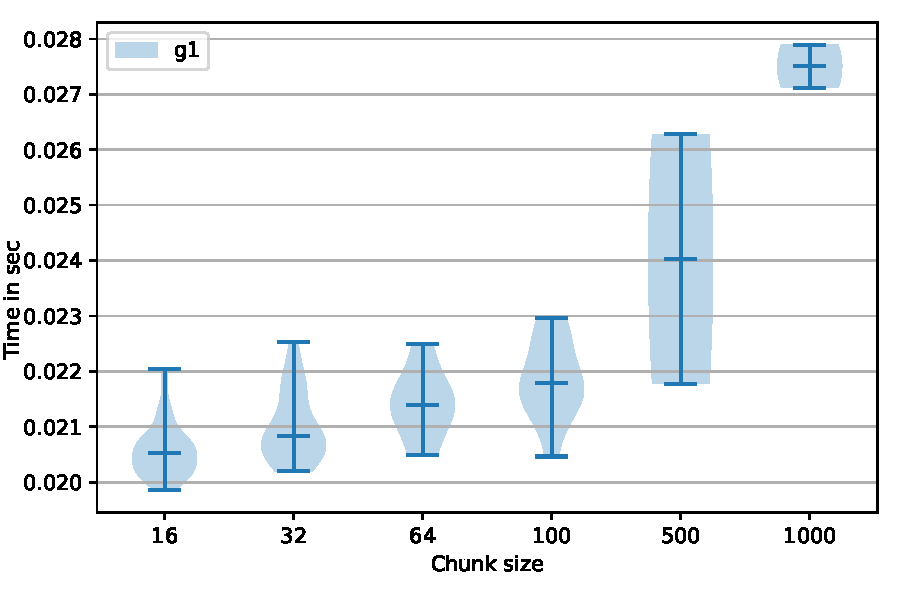
\includegraphics[width=0.45\textwidth]{data/raw/core.pdf}
\caption{Performance of \textit{core} graph querying}
\label{fig:python_core_all}
\end{figure}

\begin{figure}[h]
\centering
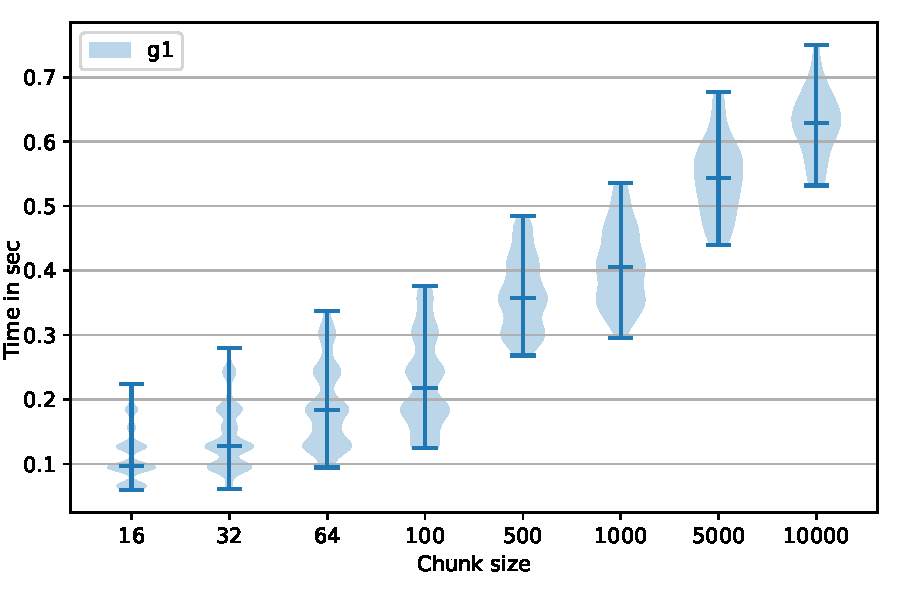
\includegraphics[width=0.45\textwidth]{data/raw/go.pdf}
\caption{Performance of \textit{go} graph querying}
\label{fig:python_go_all}
\end{figure}

\begin{figure}[h]
\centering
\includegraphics[width=0.45\textwidth]{data/raw/eclass_514en.pdf}
\caption{Performance of \textit{eclass\_514en} graph querying}
\label{fig:python_eclass_all}
\end{figure}

\begin{figure}[h]
\centering
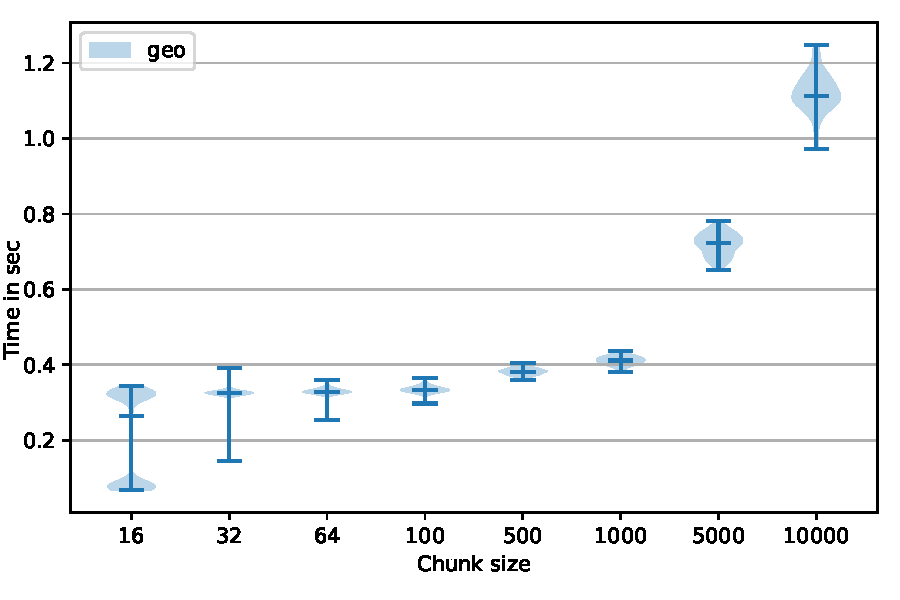
\includegraphics[width=0.45\textwidth]{data/raw/geospecies.pdf}
\caption{Performance of \textit{geospecies} graph querying}
\label{fig:python_geospecies_all}
\end{figure}

\begin{figure}[h]
\centering
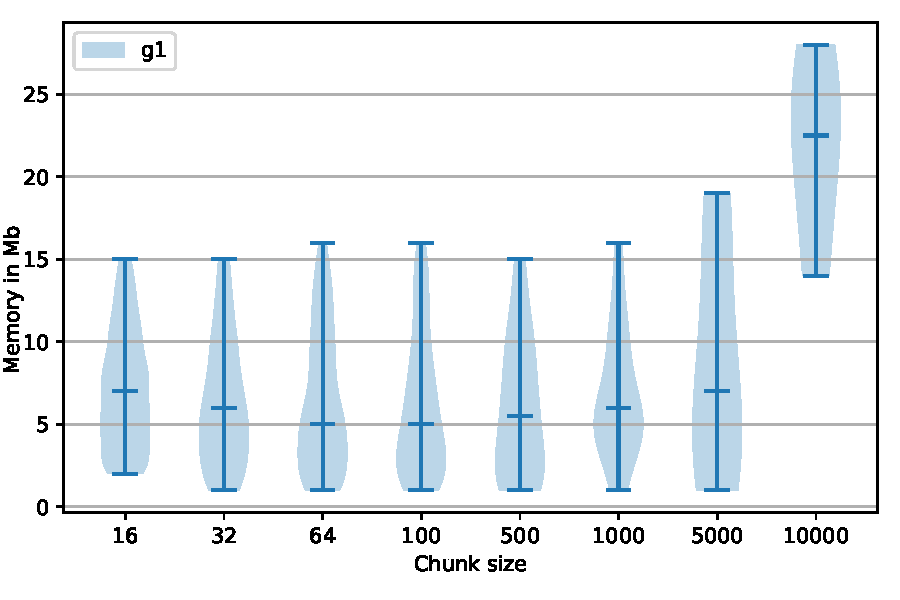
\includegraphics[width=0.45\textwidth]{data/raw/enzyme.pdf}
\caption{Performance of \textit{enzyme} graph querying}
\label{fig:python_enzyme_all}
\end{figure}

\begin{figure}[h]
\centering
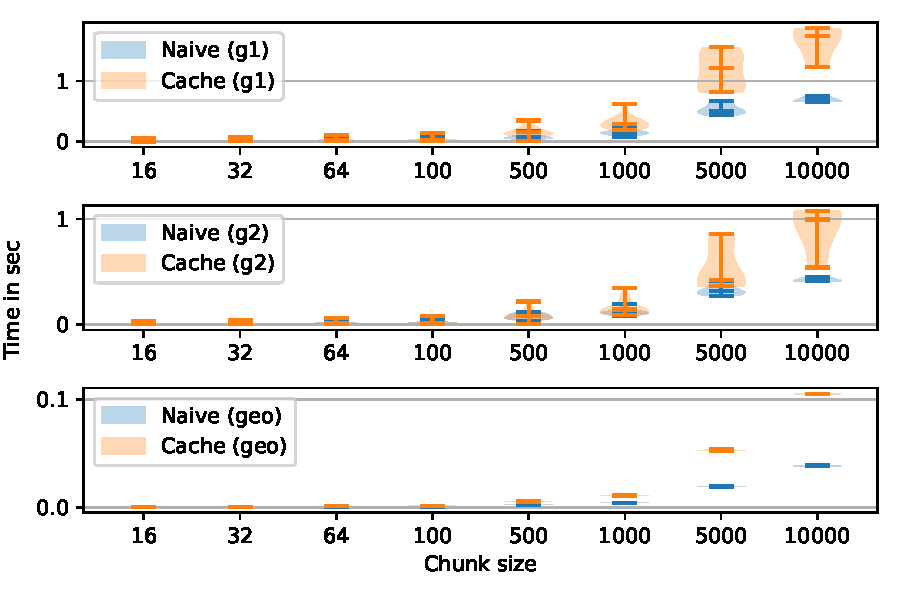
\includegraphics[width=0.45\textwidth]{data/raw/gohierarchy.pdf}
\caption{Performance of \textit{gohierarchy} graph querying}
\label{fig:python_gohierarchy_all}
\end{figure}


\begin{figure}[h]
\centering
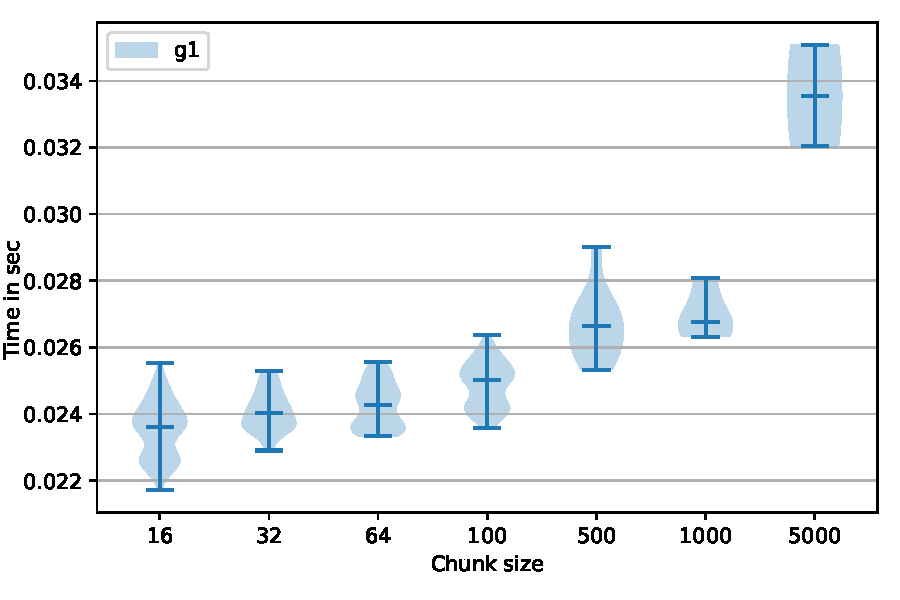
\includegraphics[width=0.45\textwidth]{data/raw/pathways.pdf}
\caption{Performance of \textit{pathways} graph querying}
\label{fig:python_pathways_all}
\end{figure}

\begin{figure}[h]
\centering
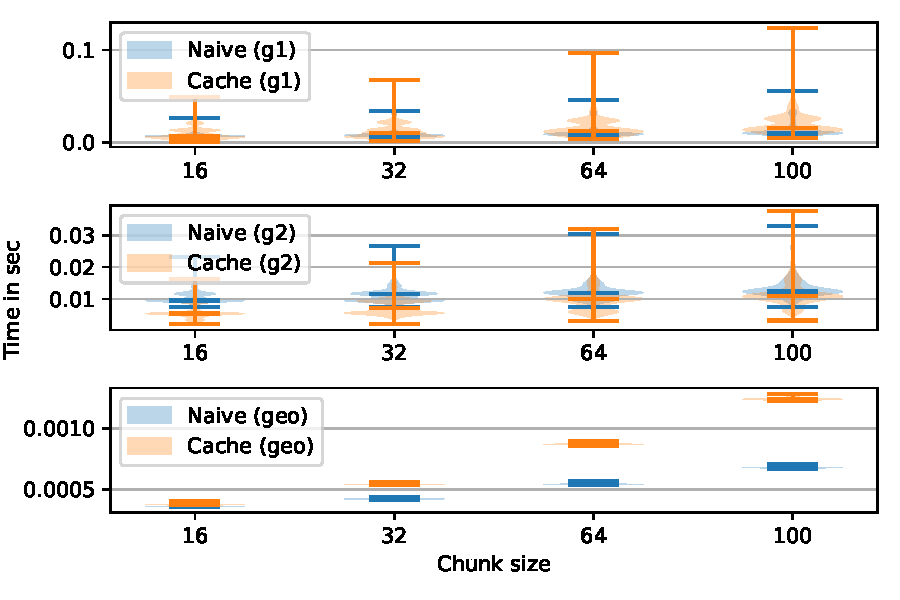
\includegraphics[width=0.45\textwidth]{data/raw/eclass_514en_4.pdf}
\caption{Performance of \textit{eclass\_514en} graph querying with small chunks}
\label{fig:python_eclass_small}
\end{figure}

\begin{figure}[h]
\centering
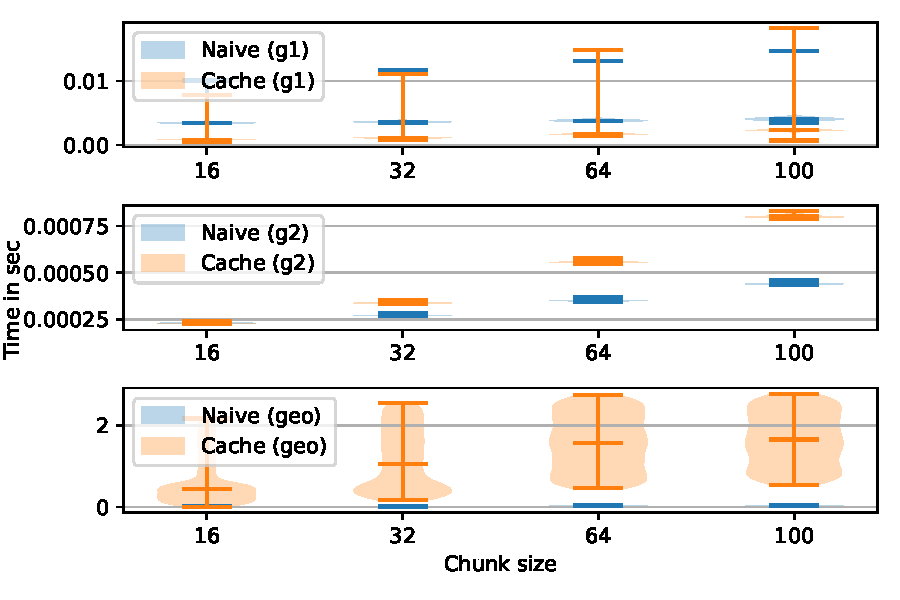
\includegraphics[width=0.45\textwidth]{data/raw/geospecies_4.pdf}
\caption{Performance of \textit{geospecies} graph querying with small chunks}
\label{fig:python_geospecies_small}
\end{figure}

\begin{figure}[h]
\centering
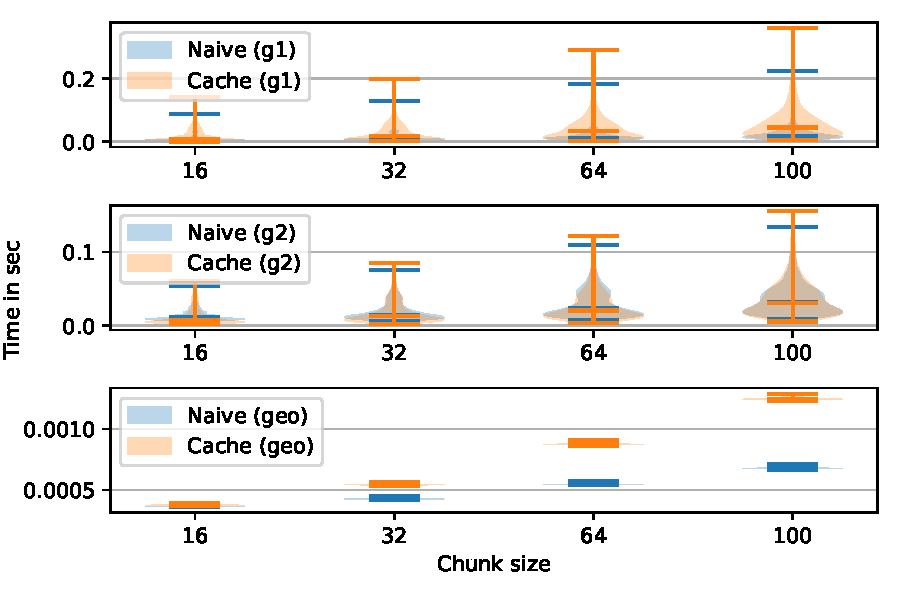
\includegraphics[width=0.45\textwidth]{data/raw/go_4.pdf}
\caption{Performance of \textit{go} graph querying with small chunks}
\label{fig:python_go_small}
\end{figure}


First of all, we can see that even for the cases when the input graph does not contain edges used in a query, the chunk processing time grows with the size of the chunk.
For example, consider the results for \textit{geo} query for all graphs except \textit{geospecies} and \textit{enzyme}.
Thus, the preliminary check of the existence of the edges of interest may improve performance.

We can also see, that the chunk processing time significantly depends on the graph structure.
For example, \textit{go} graph querying requires more than 5 seconds (fig.~\ref{fig:python_go_all}), while \textit{geospecies} graph querying requires less than 0.5 seconds (fig.~\ref{fig:python_geospecies_all}) for the chunks of size 10~000 and the query $g_1$.

The comparison of two versions of the algorithm shows that the algorithm without caching is significantly faster in almost all cases, even when the graph does not contain edges of interest.
Analysis of results for small chunks (fig.~\ref{fig:python_eclass_small}--\ref{fig:python_go_small}) shows that it is not always true.
For example, median time for algorithm with caching is slightly better than for the naive version for \textit{eclass\_514en} graph and query $g_2$ (fig.~\ref{fig:python_eclass_small}).
On the other hand, algorithm with caching is drastically slower than the naive version for \textit{geospecies} graph and $geo$ query (fig.\ref{fig:python_geospecies_small}).
At the same time, for \textit{go} graph and $g_2$ query, median time of both versions is comparable, while time for the worst queries is better for the naive version.
Moreover, caching requires additional memory in comparison with the naive version of the algorithm.
Thus we conclude, that the query results caching introduces significant overhead and does not lead to significant performance improvements.
We can also conclude that small chunk processing using the naive version is fast enough: the worst time in our experiments is about 0.2 seconds (fig.~\ref{fig:python_go_small}, query $G_1$).


As a result, we conclude that caching is not useful for multiple-source CFPQ for the evaluated cases even if one wants to process several chunks sequentially, or even process full graph chunk-by-chunk.
Thus, we believe that the naive version of the algorithm is better for implementation in a real-world graph database.





\section{CFPQ Full-Stack Support}

To provide full-stack support of CFPQ, it is necessary to choose an appropriate graph database.
It was shown by Arseniy Terekhov et al.~\cite{10.1145/3398682.3399163} that matrix-based algorithm can be naturally integrated into RedisGraph because the algorithm and the database both operate over a matrix representation of graphs.
Moreover, RedisGraph supports Cypher as a query language and there is a proposal which describes Cypher extension for context-free constraints.
Thus we chose RedisGraph as a base for our solution.


\subsection{Cypher Extension}
\label{subsec:cypher-extension}

The first thing to do is to extend the Cypher parser to support the context-free constraints.
Tobias Lindaaker proposed an extension  for context free constraints to the Cypher syntax\footnote{\label{cypher-proposal}Formal syntax specification: \url{https://github.com/thobe/openCypher/blob/rpq/cip/1.accepted/CIP2017-02-06-Path-Patterns.adoc\#11-syntax}. Access date: 19.07.2020.}, which is not implemented in the Cypher parsers yet.

This extension introduces path patterns, which are a powerful alternative to the original Cypher relationship patterns.
Path patterns allow one to express regular constrains over the basic patterns such as relationship and node patterns.
Like relationship patterns, they can be specified in the \texttt{MATCH} clause.

The feature which allows one to specify context-free constraints is \textit{named path patterns}: a path pattern can be assigned a name which can be used in other patterns or within the same pattern.
Named patterns is defined in the \texttt{PATH PATTERN} clause.
Using this feature, the structure of queries is pretty similar to a grammar in the Extended Backus-Naur Form (EBNF)~\cite{EBNF_ISO}.

\begin{algorithm}[t]
\floatname{algorithm}{Listing}
\begin{algorithmic}[1]
\caption{Query based on the example grammar $G_1$ written in Cypher with path patterns}
\label{lst:cypher_example}
\State PATH PATTERN S = ()-/ [:c $\sim$S :d] | [:c (:y) :d] /->()
\State MATCH (v:x)-[:a | :c]->()-/ :b $\sim$S /->(to)
\State RETURN v, to
\end{algorithmic}
\end{algorithm}


An example of a query which uses named path patters is presented in listing~\ref{lst:cypher_example}.
This query is based on the context-free grammar $G_1$.
Namely, the path pattern \texttt{S} specifies exactly the same constraint as the grammar $G_1$.
The \texttt{MATCH} clause consists of the relation pattern \texttt{[:a | :c]} and the path pattern \texttt{/:b $\sim$S/}, and this path pattern references the named pattern \texttt{S}.
The constraint specifies that a path of interest starts in a vertex labelled \texttt{x}, goes through an edge labelled either \texttt{a} or \texttt{c}, then the rest of the path is constrainted by a path pattern which starts with an edge \texttt{b} and follows with a path matched with \texttt{S}.
The \texttt{RETURN} clause specifies what the result of the query is supposed to be.
For the example graph $D_1$, this query returns the set of vertex pairs $\{(0, 4), (0, 5)\}$.

RedisGraph database supports a subset of the Cypher language and uses \texttt{libcypher-parser}\footnote{The \texttt{libcypher-parser} is an open-source parser library for Cypher query language. GitHub repository of the project: \url{https://github.com/cleishm/libcypher-parser}. Access date: 19.07.2020.} library to parse queries.
We extend this library with the new syntax described in the proposal.
Note that we implement\footnote{The modified libcypher-parser library with support of syntax for path patterns: \url{https://github.com/YaccConstructor/libcypher-parser}. Access date: 19.07.2020.} the complete syntax extension, not only the part necessary for simple CFPQ.

\subsection{RedisGraph Extension}

We implemented the multiple-source algorithm in the RedisGraph.
We partially supported the proposed syntax extension in RedisGraph query execution engine so that one can specify the labels of edges and vertices and use named path patterns.

Processing the input as a whole may require a lot of memory.
RedisGraph implements lazy evaluation: it creates execution strategy in terms of elementary operations each of which processes the input sequentially in \emph{chunks}.
This reduces memory consumption so that it does not depend on the input size which is crucial when dealing with big real-world graphs.
However processing chunks comes with a time overhead.
By changing the size of a chunk, a developer may adjust the ratio between the time and memory consumption so that it fits their needs.

We use subsets of the start vertices as chunks since it is most natural in the multiple source algorithm.
We study how the size of a chunk affects the performance in the evaluation.

\subsection{Evaluation}

For RedisGraph evaluation, we used a PC with Ubuntu 18.04 installed.
It has Intel Core i7-6700 CPU, 3.4GHz, and DDR4 64Gb RAM.
RedisGraph with our extensions is installed\footnote{Sources of RedisGraph database with full-stack CFPQ support:\url{https://github.com/YaccConstructor/RedisGraph/tree/path_patterns_dev}. Access date: 19.07.2020.}.

\subsubsection{Data Preparation}

We use the graphs and respective queries $g_1$ and $geo$ from~\cite{10.1145/3398682.3399163} to evaluate the RedisGraph-based solution.
The graphs are loaded into the RedisGraph database so that each vertex has a unique property \verb|id| in the range $[0, \ldots, |V|-1]$, where $|V|$ is a number of vertices in the graph to load.
This allows us to generate queries for a start vertex set with specific size using templates.
The template for the $g_1$ query is provided in listing~\ref{lst:query_pattern_g1}.
Here \texttt{\{id\_from\}} and \texttt{\{id\_to\}} are placeholders for the lower and the upper bounds for \verb|id|.

\begin{algorithm}
\floatname{algorithm}{Listing}
\begin{algorithmic}[1]
\caption{Cypher query pattern for $g_1$}
\label{lst:query_pattern_g1}
\State PATH PATTERN S =  \par
 \hskip\algorithmicindent ()-/ [<:SubClassOf [$\sim$S | ()] :SubClassOf] \par
 \hskip\algorithmicindent | [<:Type [$\sim$S | ()] :Type] /->()
\State MATCH (src)-/ $\sim$S /->()
\State WHERE \{id\_from\} <= src.id and src.id <= \{id\_to\}
\State RETURN count(*)
\end{algorithmic}
\end{algorithm}

We implemented a query generator for the queries $g_1$ and $geo$ to create concrete queries for all the start sets which are used in the previous experiment.


\subsubsection{Evaluation Results}

We use $geo$ query for \textit{geospecies} graph as one of the hardest queries, and $g_1$ query for other graphs.
We measure time and memory consumption for each start set.

\begin{figure}[h]
\centering
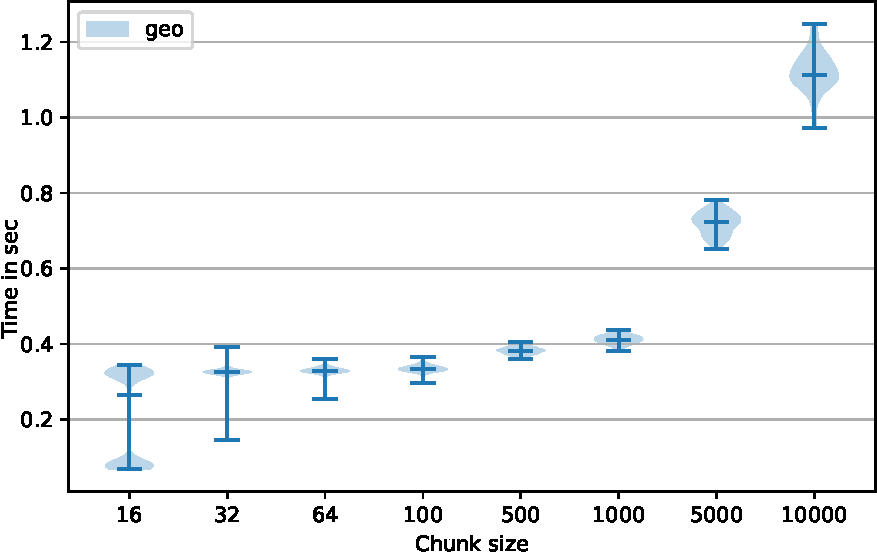
\includegraphics[width=0.41\textwidth]{data/raw_redis/geospecies.pdf}
\caption{RedisGraph performance on \textit{geospecies} graph}
\label{fig:redis_geospecies_all}
\end{figure}

\begin{figure}[h]
\centering
\includegraphics[width=0.41\textwidth]{data/raw_redis/eclass_514en.pdf}
\caption{RedisGraph performance on \textit{eclass\_514en} graph}
\label{fig:redis_eclass_all}
\end{figure}

The execution time for all sets, except the set of size 10~000 for \textit{geospecies} graph (fig.~\ref{fig:redis_geospecies_all}), is less than 1 second.
Moreover, for smaller graph (\textit{eclass\_514en}), processing time is less than 0.2 second for all chunks (fig.~\ref{fig:redis_geospecies_all}).

Memory consumption for the big graphs \textit{eclass\_514en} and \textit{geospecies} is presented in figures~\ref{fig:redis_memory_eclass} and~\ref{fig:redis_memory_geospecies} respectively.
The amount of memory used depends on the graph and the query, but RedisGraph uses less that 50Mb of RAM to process graphs with relatively small chunks ($\leq 1000$).
Note that RedisGraph includes memory management system, thus we measured all allocated memory, not only the memory really used for the query evaluation.
As a result, we can conclude that the multiple-source CFPQ is significantly more memory efficient than creation of the complete reachability index and its filtering: processing the set of size 10~000 on \textit{geospecies} graph requires less than 200Mb, while full index creation requires 16Gb~\cite{10.1145/3398682.3399163}.

\begin{figure}[t]
\centering
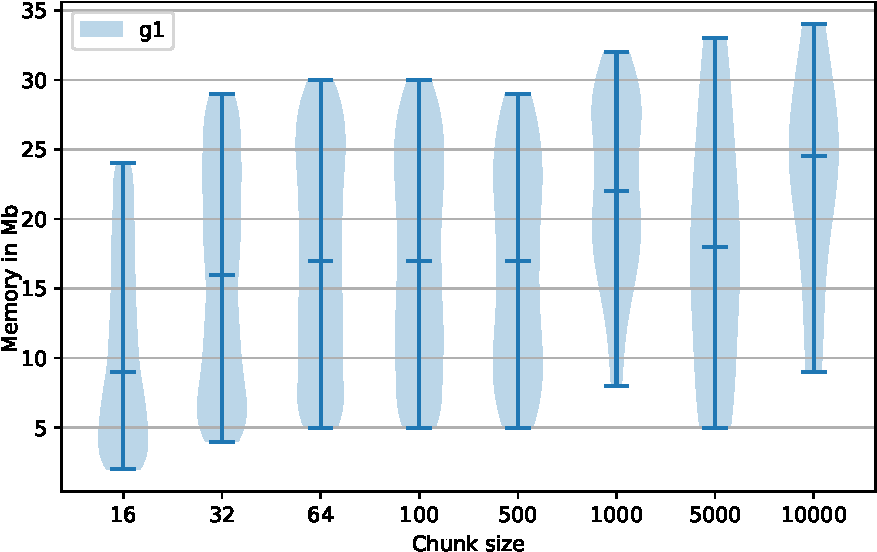
\includegraphics[width=0.41\textwidth]{data/raw_memory/eclass_514en.pdf}
\caption{Memory consumption on \textit{eclass\_514en}}
\label{fig:redis_memory_eclass}
\end{figure}

\begin{figure}[t]
\centering
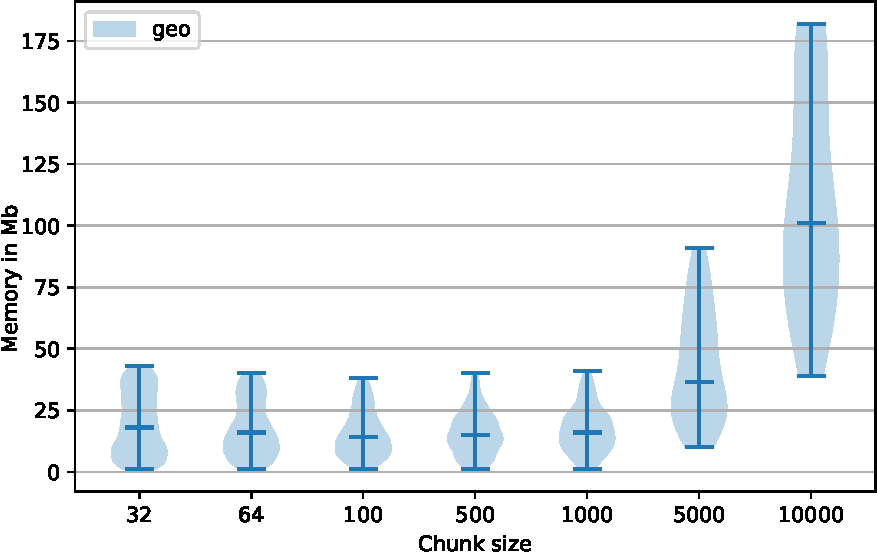
\includegraphics[width=0.41\textwidth]{data/raw_memory/geospecies.pdf}
\caption{Memory consumption on \textit{geospecies}}
\label{fig:redis_memory_geospecies}
\end{figure}

We also evaluate how chunking affects the performance on the all-pairs reachability problem.
We fix the size of a chunk to be 1000 for graphs of different sizes and measure time and memory required to process queries.
Namely, we evaluate the query which is similar to the query from the previous scenario, but it does not constraint vertices ids (it does not have the \texttt{WHERE} clause).
We measure total processing time (in seconds) and total required memory (in Mb).
Also, we compare our solution with the results of Arseniy Terekhov et al. from~\cite{10.1145/3398682.3399163} in which the Azimov's algorithm was naively integrated with RedisGraph without support of lazy query evaluation and query language.
Similar hardware and the same input graphs and queries were used.
Results are provided in table~\ref{tbl:redis_full_graph_processing}.

{\setlength{\tabcolsep}{0.25em}
\begin{table}
{
\caption{Full graph processing with chunks of size 1000}
\label{tbl:redis_full_graph_processing}
\small
\rowcolors{3}{black!2}{black!10}
\begin{tabular}{|l|c|c|c|c|c|c|}
\hline
\multirow{2}{*}{Graph} & \multirow{2}{*}{\#V} & \multirow{2}{*}{\#E} & \multirow{2}{*}{Q} & \multicolumn{2}{c|}{Chunks}  &  {Mono~\cite{10.1145/3398682.3399163}}  \\
                       &                      &                      &                        & T (sec)  & Mem (Mb) &  T (sec)\\
\hline
\hline
core                   & 1323                 & 4342                 & $g_1$                  & 0.003  & 2                  &  0.004 \\
pathways               & 6238                 & 18 598               & $g_1$                  & 0.031  & 6                  &  0.011 \\
gohierarchy            & 45 007               & 980 218              & $g_1$                  & 0.847  & 62                  &  0.091 \\
enzyme                 & 48 815               & 109 695              & $g_1$                  & 0.698  & 13                  &  0.018 \\
eclass\_514en          & 239 111              & 523 727              & $g_1$                  & 18.825 & 35                   &  0.067 \\
geospecies             & 450 609              & 2 311 461            & $geo$                  & 80.979 & 196                  &  7.146 \\
go                     & 272 770              & 534 311              & $g_1$                  & 72.034 & 40                  &  0.604 \\
\hline
\end{tabular}
}
\end{table}
}

Although chunk-by-chunk processing is slower, it still requires reasonable time.
Moreover, if the chunk size is comparable with the graph size (\textit{core} and \textit{pathways} graphs), then the execution time is comparable with the monolithic processing.
Thus one can decrease execution time by increasing the chunk size.
On the other hand, even with relatively small chunks (\textit{eclass\_514}, \textit{go} and \textit{geospecies} graphs), when for chunk-by-chunk processing is 100 times slower, our results are still reasonable for some cases.
For example, it requires over 70 times less time for \textit{geospecies} graph processing than the solution of Jochem Kuijpers et al.~\cite{Kuijpers:2019:ESC:3335783.3335791} which is based on Neo4j and requires more than 6000 seconds.
Moreover, while the solution from~\cite{10.1145/3398682.3399163} requires huge amount of memory (more than 16Gb for \textit{geospecies} graph and $geo$ query), our solution requires only 196Mb.
We argue, that our solution is more suitable for general-purpose graph databases.
First of all, the core scenario when the set of start vertices is relatively small can be handled efficiently.
Second, all-pairs reachability, which is not a massive case, can be solved in reasonable time with low memory consumption.
One can easily tune our solution to get the optimal time and memory consumption for their specific case.

%\section{Evaluation}

For performance analysis of proposed solution we evaluated some most common graph algorithms using real-world sparse matrix data. 
As a baseline for comparison we chose LAGraph~\cite{szarnyas2021lagraph} in connection with SuiteSparse~\cite{10.1145/3322125} as a CPU tool, Gunrock~\cite{7967137} and GraphBLAST~\cite{yang2019graphblast} as a Nvidia GPU tools. 
Also, we tested algorithms on several devices with distinct OpenCL vendors in order to validate portability of the proposed solution. 
In general, these evaluation intentions are summarized in the following research questions. 

\vspace{0.2cm}
\begin{itemize}
    \item[\textbf{RQ1}] What is the performance of the proposed solution relative to existing tools for both CPU and GPU analysis?
    
    \item[\textbf{RQ2}] What is the portability of the proposed solution with respect to various device vendors and OpenCL runtimes?
\end{itemize}

\subsection{Evaluation Setup}

For evaluation, we use a PC with Ubuntu 20.04 installed, which has 3.40Hz Intel Core i7-6700 4-core CPU, DDR4 64Gb RAM, and Nvidia GeForce GTX 1070 GPU with 8Gb VRAM. 
Host programs were compiled with GCC 9.3.0 compiler. Programs using CUDA were compiled with GCC 8.4.0 and Nvidia NVCC 10.1.243 compiler.
Release mode and maximum optimization level was enabled for all tested programs. 
Data loading time, preparation, format transformations and host-device initial communications are excluded from time measurements. 
All tests are averaged across 10 runs.
Additional warm-up run for each test execution is excluded from measurements.

\subsection{Graph Algorithms}

For preliminary study \textit{breadth-first search} (bfs) and \textit{triangles counting} (tc) algorithms were chosen, since they allows analyse the performance of \textit{vxm} and \textit{mxm} operations, rely heavily on \textit{masking}, and utilize \textit{reduction} or \textit{assignment}. 
BFS implementation utilizes automated vector storage from sparse to dense switch and only \textit{}{push optimization}. 
TC implementation uses masked \textit{mxm} of source lower-triangular matrix with second transposed argument.

\subsection{Dataset}

Nine graph matrices were selected from the Sparse Matrix Collection at University of Florida~\cite{dataset:10.1145/2049662.2049663}. 
Information about graphs is summarized in Table~\ref{dataset:info}. 
All datasets are converted to undirected graphs. 
Self-loops and duplicated edges are removed.

\begin{table}[htbp]
\caption{Dataset description.} 
\begin{center}
    \rowcolors{2}{black!2}{black!10}
    \begin{tabular}{|l|r|r|r|}
    \hline
    Dataset & Vertices  & Edges & Max Degree \\
    \hline
    \hline
    coAuthorsCiteseer & 227.3K &   1.6M &    1372 \\
    coPapersDBLP      & 540.4K &  30.4M &    3299 \\
    hollywood-2009    &   1.1M & 113.8M &  11,467 \\
    roadNet-CA        &   1.9M &   5.5M &      12 \\
    com-Orkut         &     3M &   234M &   33313 \\
    cit-Patents       &   3.7M &  16.5M &     793 \\
    rgg\_n\_2\_22\_s0 &   4.1M &  60.7M &      36 \\
    soc-LiveJournal   &   4.8M &  68.9M &  20,333 \\
    indochina-2004    &   7.5M & 194.1M & 256,425 \\
    \hline
    \end{tabular}
    \label{dataset:info}
\end{center}
\end{table}

\subsection{Results}

Table~\ref{results} presents results of the evaluation and compares performance of Spla against other tool on different execution platforms.
Tools are grouped by the type of the device for the execution, where either Nvidia GPU or Intel CPU are used. 
Cell left empty if tested tool failed to analyse graph due to \textit{out of memory} exception.

In general, Spla BFS shows acceptable performance, especially on graphs with large vertex degree, such as soc-LiveJournal and com-Orkut.
On graphs roadNet-CA and rgg it has a significant performance drop due to the nature of underlying algorithms and data structures. 
Firstly, library utilizes immutable data buffers. Thus, iteratively updated dense vector of reached vertices must be copied for each modification, what dominates the performance of the library on a graph with large search depth. 
Secondly, Spla BFS does not utilise \textit{pull optimization}, what is critical in a graph with relatively small search frontier. 

Spla TC has a good performance on GPU, which is better in all cases that reference SuiteSparse solution. 
But in most tests GPU competitors, especially Gunrock, show smaller processing times. 
GraphBLAST shows better performance as well. 
Library utilises masked SpGEMM algorithm, the same as in GraphBLAST, but without \textit{identity} element to fill gaps. 
Library explicitly stores all non-zero elements, and uses mask to reduce only non-zero while evaluating dot products of rows and columns. 
What causes extra divergence inside work groups. 
On Intel device Spla shows better performance compared to SuiteSparse on com-Orkut, cit-Patents and soc-LiveJournal. 
A possible reason is the large lengths of processed rows and columns in the product of matrices.

Gunrock shows nearly best average performance due to its specialized and optimized algorithms.
Also, it has good time characteristics on a mentioned earlier roadNet-CA and rgg in BFS algortihm. 
GraphBLAST follows Gunrock and show good performance as well. 
But it runs out of memory on a two significantly large graphs con-Orkut and indochina-2004. 
Spla does not rut out of memory on any test due to simplified storage scheme.

\begin{table}[htbp]
\caption{Graph algorithms evaluation results.\\Time in milliseconds (lower is better).} 
\begin{center}
    \begin{tabular}{|l|r|r|r|r|r|}
    \hline
    \multirow{2}{*}{Dataset} & \multicolumn{3}{c|}{Nvidia} & \multicolumn{2}{c|}{Intel} \\
    \cline{2-6}
    & GR & GB & SP & SS & SP \\
    \hline
    \hline
    \multicolumn{6}{|c|}{BFS} \\
    \hline
    \rowcolor{black!10} hollywood-2009    &  20.3 &  82.3 &   36.9 &   23.7 &   303.4 \\
    \rowcolor{black!2 } roadNet-CA        &  33.4 & 130.8 & 1456.4 &  168.2 &   965.6 \\
    \rowcolor{black!10} soc-LiveJournal   &  60.9 &  80.6 &   90.6 &   75.2 &  1206.3 \\
    \rowcolor{black!2 } rgg\_n\_2\_22\_s0 &  98.7 & 414.9 & 4504.3 & 1215.7 & 15630.1 \\
    \rowcolor{black!10} com-Orkut         & 205.2 & -- -- &  117.9 &   43.2 &   903.6 \\
    \rowcolor{black!2 } indochina-2004    &  32.7 & -- -- &  199.6 &  227.1 &  2704.6 \\
    \hline
    \hline
    \multicolumn{6}{|c|}{TC} \\
    \hline
    \rowcolor{black!10} coAuthorsCiteseer &   2.1 &    2.0 &    9.5 &    17.5 &    64.9 \\
    \rowcolor{black!2 } coPapersDBLP      &   5.7 &   94.4 &  201.9 &   543.1 &  1537.8 \\
    \rowcolor{black!10} roadNet-CA        &  34.3 &    5.8 &   16.1 &    47.1 &   357.6 \\
    \rowcolor{black!2 } com-Orkut         & 218.1 & 1583.8 & 2407.4 & 23731.4 & 15049.5 \\
    \rowcolor{black!10} cit-Patents       &  49.7 &   52.9 &   90.6 &   698.3 &   684.1 \\
    \rowcolor{black!2 } soc-LiveJournal   &  69.1 &  449.6 &  673.9 &  4002.6 &  3823.9 \\
    \hline
    \hline
    \multicolumn{6}{l}{Tools: Gunrock (GR), GraphBLAST (GB), SuiteSparse (SS), Spla (SP).} \\
    \end{tabular}
    \label{results}
\end{center}
\end{table}
 
% Two GPU

% \begin{table}[htbp]
%     \caption{Table Type Styles}
%     \begin{center}
%     \begin{tabular}{|c|c|c|c|}
%     \hline
%     \textbf{Table}&\multicolumn{3}{|c|}{\textbf{Table Column Head}} \\
%     \cline{2-4} 
%     \textbf{Head} & \textbf{\textit{Table column subhead}}& \textbf{\textit{Subhead}}& \textbf{\textit{Subhead}} \\
%     \hline
%     copy& More table copy$^{\mathrm{a}}$& &  \\
%     \hline
%     \multicolumn{4}{l}{$^{\mathrm{a}}$Sample of a Table footnote.}
%     \end{tabular}
%     \label{tab2}
%     \end{center}
% \end{table}

\section{Conclusion}

In this paper we present a library for sparse Boolean linear algebra which implements such basic operations as matrix-matrix multiplication and element-wise matrix-matrix addition in both Cuda and OpenCL.
Evaluation shows that our Boolean-specific implementations faster and require less memory than generic, not the Boolean optimized, operations from state-of-the-art libraries. 
Thus, the specialization of operations for this data type makes sense. 

The first direction of the future work is to integrate all parts (OpenCL and Cuda backends) into a single library and improve its documentation and prepare to publish.
Moreover, it is necessary to extend the library with other operations, including matrix-vector operations, masking, and so on.
As a result a Python package should be published.

Another important step is to evaluate the library on different algorithms and devices.
Namely, algorithms for RPQ and CFPQ should be implemented and evaluated on related data sets.
Also, it is necessary to evaluate OpenCL version on FPGA which may require additional technical effort and code changes.

Finally, we plan to discuss with GraphBLAS community possible ways to use our library as a backend for GraphBLAST or SuiteSparse in case of Boolean computations.
Moreover, it may be possible to use implemented algorithms as a foundation for generalization to arbitrary semirings.


\section*{Acknowledgements}
The research was supported by the Russian Science Foundation, grant \textnumero 18-11-00100.

We thank Roi Lipman for his help with investigation of the RedisGraph internals and pointing out the impractical memory consumption of the original Azimov's algorithm which gave us the motivation to develop the presented solution.

We thank Ekaterina Verbitskaia for the fruitful discussion and feedback which helped us to improve the paper.

%Anonimus reviewers !!!

\balance

%%
%% The next two lines define the bibliography style to be used, and
%% the bibliography file.
\bibliographystyle{ACM-Reference-Format}
\bibliography{multiple-source-matrix-cfpq}

%%
%% If your work has an appendix, this is the place to put it.
%% Please note that all the content must fit within the page limits, including any appendices.
%\appendix
%
%\section{Research Methods}
% ...

\end{document}
\endinput




